\chapter{The Zone}
\label{ch:zone}

The Zone is an execution context associated to a code block. It represents the asynchronous extension of a scope. Like a scope, the Zone can contain other Zones.

% The primordial purpose of Zones is to answer the lack of context persistency when submitting asynchronous task. Zones allow to store key-value bindings and holds across asynchronous execution. Hence, they make it possible to share information between asynchronous executions. Because the key-value bindings may be shared by concurrent executions, they must stay immutable to avoid race conditions. However, it is still possible to locally add more key-value bindings by creating a new Zone with additional bindings. It is safe since concurrent executions won't be affected by the local context modification. Furthermore, it is still possible in Java to bypass this limitation, modifiying the content of immutable references.

The primordial purpose of Zones is to provide uniformity across asynchronous executions. It specifies constant key-value bindings accessible anywhere in the context (Zone values), task to execute when entering (cross-in hook) or exiting (cross-out hook) a Zone and hooks around synchronous (internal hook) and asynchronous (asynchronous hook) task submission. Those around hooks make it possible to manipulate the tasks that gets executed inside the Zone. While they are not essential to the concept of Zone itself, the opportunity to implement them naturally appears in a Zone implementation since the realization requires asynchronous submission hooks (see section \ref{sec:realization}). The Zone can then simply make these hooks accessible on its interface.

\section{Model}

As illustrated in figure \ref{fig:zpn}, the Zone can be understood as an extension to Petri net that allows to capture the tokens flow.

\begin{figure}
  \centering
  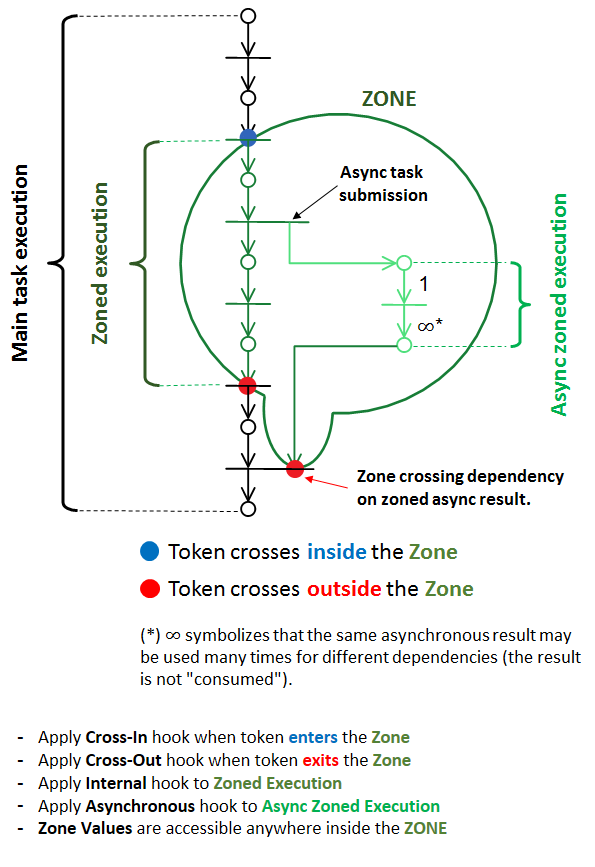
\includegraphics[width=\textwidth]{zone-pn-new}
  \caption{Zone on Petri net}
  \label{fig:zpn}
\end{figure}

More formally, given a Petri net $PN = (P, T, F)$ with $P$ the set of places, $T$ the set of transitions and $F$ the set of flows from $P$ to $T$ or $T$ to $P$: $F \subseteq (P \times T) \cup (T \times P)$, a Zone $Z$ is a subset $Z \subseteq P$ such that:

$$\forall Z_1, Z_2 \exists Z_0 \text{ s.t. } Z_1 \subseteq Z_0 \land Z_2 \subseteq Z_0 $$

$$\forall Z_1, Z_2 (Z_1 \cap Z_2 \neq \emptyset) \Rightarrow [(Z_1 \subseteq Z_2) \lor (Z_2 \subseteq Z_1)] $$

Which more simply means: there exists a \emph{root} Zone enclosing all Zones and Zones can contain other Zones, but cannot intersect otherwise (figure \ref{fig:zinter}).

\begin{figure}[h]
  \centering
  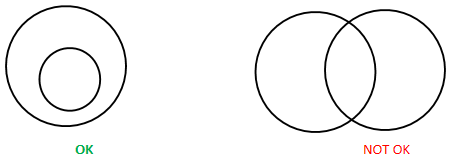
\includegraphics[width=\textwidth]{zone-intersect}
  \caption{Zone intersection}
  \label{fig:zinter}
\end{figure}

The key-value bindings defined by the Zone are accessible from any place inside that Zone. The crossing hooks are triggered whenever a token crosses a Zone boundary.

The Zone identifies a crossing event when a token of the Petri net moves between two places that do not belong to the same Zones (see crossing algorithm in section \ref{sec:cross-res}). For more liberty in the crossing hooks, tokens may carry nothing (void tokens) an error (error tokens) or the result of a zoned task (result tokens). In Java, the tokens are implemented as simple objects containing a result, an error value or nothing.

In order to know which Zone originated a token, they are wrapped as zoned tokens. A zoned token is simply a tuple containing a token and its source Zone.

Operations on token while crossing Zone boundaries are described by the Zone's crossing hooks.
The presence of around hooks defined in the Zone allows even more capabilities. However, unlike the crossing hooks, these around hooks are closer to an implementation feature than a primary effect of the model.

\section{Terminology}

In order to ease further discussion and presentation of the Zone, this section gives a small glossary of the essential terms used in the Zone.


\textbf{Task} represents the very general concept of ``something the program has to do''. More formally, a task is a procedure with some input and zero or one output. For example, \lstinline{Runnable} is a task with no input, no output. A method call is a task with method's arguments as input and method's return value as output.

\textbf{Zoned Token} is a tuple containing a token with its origin Zone. Zoned tokens are used as input to the crossing resolution algorithm (see section \ref{sec:cross-res}).

\textbf{Zoned Task} is the result of binding a task to a Zone. A Zoned task behaves like a task but accepts and return only zoned tokens. For instance a task expressed in Java by
\begin{lstlisting}
Function<T, U> task;
\end{lstlisting}
Is associated to a zoned task represented by
\begin{lstlisting}
Function<ZonedToken<T>, ZonedToken<U>> zonedTask;
\end{lstlisting}

\textbf{Zone Stack} is the stack of all enclosing zones at a given point of the program execution. Innermost Zone is considered to be at the top of the Zone Stack. If no Zone is defined, the current Zone is considered to be the default root Zone. For example :

\begin{lstlisting}
(new ZoneA()).run(() -> {
  /*
   * Zone stack here is:
   * ZoneA, ROOT_Zone
   */
   (new ZoneB()).run(() -> {
     /*
      * Zone stack here is:
      * ZoneB, ZoneA, ROOT_ZONE
      */
   });
});
/*
 * Zone stack here is back to:
 * ROOT_ZONE
 */
\end{lstlisting}

\section{Crossing Resolution}
\label{sec:cross-res}

The crossing principle is the original feature of the Zone. The base mechanism is simple. Value outputted by zoned tasks are \emph{zoned tokens}. When the value of a zoned token is used, it is extracted out of the zoned token to the current Zone, triggering the crossed Zones crossing hook.

Multiple cases can occur with the crossing mechanism. Especially in the Java implementation, where it is possible to keep and carry around references to already bound tasks, a token extraction can arise in unexpected contexts. Rather than relying on visibility restrictions to prevent such unusual cases to occur, the crossing resolution properly defines how the model behaves under such circumstances.

For better understanding, keep in mind that at the bottom of every single Zone stack, there is the Root Zone. The Root Zone can be seen as the Zone with no hooks and values enclosing the whole program.

In the given code examples, \lstinline{new Zone()} creates a Zone whose parent is the enclosing Zone. For instance:

\begin{lstlisting}
Zone zone1 = new Zone();
Zone zone2;
zone1.run(() -> {
  // inside zone1
  zone2 = new Zone();
});

assert(zone1.getParent() == ROOT_ZONE);
assert(zone2.getParent() == zone1);
\end{lstlisting}

The crossing resolution algorithm always receives three parameters :

\begin{enumerate}
\item The source Zone
\item The destination Zone
\item The crossing Token
\end{enumerate}

The crossing token is \emph{not} a zoned token. The zoned tokens used by the framework provide the source Zone of the crossing resolution algorithm and the crossing token. The destination Zone is the current Zone of the extraction.

The crossing algorithm is divided in four steps:
\begin{enumerate}
\item Collect the Zone stack of the source Zone and the destination Zone to get the source stack and the destination stack.
\item Eliminate the common bottom part of the stacks. Recall that every Zone is a (indirect) child of the Root Zone, hence both stacks have at least one Zone in common. The idea of this step is to find the closest common enclosing the source and destination Zones: the \emph{join Zone}.
\item Cross out the rest of the source stack in top-down order with the crossing token. This means calling each crossing hooks of the crossed Zone with the crossing token as argument.
\item Cross-in the rest of the destination stack in down-top order with the crossing token.
\end{enumerate}

Let's see some concrete example of crossing resolutions.

\subsection*{Base case}

The common case of zoned execution is running code in a child Zone.

\begin{lstlisting}
// current Zone = some Zone

(new Zone()).run(() -> {
  // current Zone = new Zone

  // do zoned stuff here
});
\end{lstlisting}

When the code zoned in new Zone starts, the cross algorithm executes in a very simple configuration.

\begin{tabular}{| l | l |}
\hline
\textbf{Source Zone} & Some Zone
\\ \hline
\textbf{Destination Zone} & New Zone
\\ \hline
\textbf{Join Zone} & Some Zone
\\ \hline
\multicolumn{2}{l}{}
\\ \hline
\textbf{Source Zone Stack} & Some Zone :: ROOT\_ZONE
\\ \hline
\textbf{Destination Zone Stack} & New Zone :: Some Zone :: ROOT\_ZONE
\\ \hline
\textbf{Common Part} & Some Zone :: ROOT\_ZONE
\\ \hline
\multicolumn{2}{l}{}
\\ \hline
\textbf{Pruned Source Stack} & $\emptyset$
\\ \hline
\textbf{Pruned Destination} & New Zone
\\ \hline
\end{tabular}

Since the join Zone is the source Zone, the left source stack after step 2 is empty. Step 3 of the algorithm has no effect. No cross-out hook is applied, only one cross-in, of the destination Zone, is executed.

When the code zoned in new Zone ends, the cross algorithm executes in the dual configuration, still simple:

\begin{tabular}{| l | l |}
\hline
\textbf{Source Zone} & New Zone
\\ \hline
\textbf{Destination Zone} & Some Zone
\\ \hline
\textbf{Join Zone} & Some Zone
\\ \hline
\multicolumn{2}{l}{}
\\ \hline
\textbf{Source Zone Stack} &  New Zone :: Some Zone :: ROOT\_ZONE
\\ \hline
\textbf{Destination Zone Stack} & Some Zone :: ROOT\_ZONE
\\ \hline
\textbf{Common Part} & Some Zone :: ROOT\_ZONE
\\ \hline
\multicolumn{2}{l}{}
\\ \hline
\textbf{Pruned Source Stack} & New Zone
\\ \hline
\textbf{Pruned Destination} & $\emptyset$
\\ \hline
\end{tabular}

The join Zone remains the source Zone, but the left destination stack is emptied by step 2. Step 3 executes one cross out (from the source Zone), step 4 executes no cross-in. To summarize, in this case, a cross in is executed when entering the new Zone, a cross out is executed when entering the old Zone. So far, so good.

\subsection*{Running in parent Zone from child Zone}

This case allows to see that starting code execution in a Zone does not necessarily implies crossing in.

\begin{lstlisting}
// keeps reference to parent Zone
Zone parent = new Zone();

parent.run(() -> {
  // inside Zone parent
  Zone child = new Zone();
  child.run(() -> {
    // inside Zone child

    // this is the point of interest
    parent.run(() -> {
      // Zoned code here !!
    });
  });
});
\end{lstlisting}

When the code zoned in parent (at the point of interest) starts, the cross algorithm executes with the opposite configuration of the base case:

\begin{tabular}{| l | l |}
\hline
\textbf{Source Zone} & Child Zone
\\ \hline
\textbf{Destination Zone} & Parent Zone
\\ \hline
\textbf{Join Zone} & Parent Zone
\\ \hline
\end{tabular}

When entering the Zone, the argument pattern is the same as when ending in the base case. Hence one cross-out will be executed, no cross-in. Reversely, one cross-in and no cross-out is executed when ending in the Zone.
It is interesting to note that running in parent does not add layers on the Zone stack, but effectively pops the child Zone out of it. Adding once more the parent Zone on the Zone stack would not make sense, since the parent is an instantiation of a Zone, defining its own Zone stack (the context in which it was instantiated).


\subsection*{Entering a Sibling Zone}

This last example shows how, in one single crossing resolution, can both cross-in and cross-out hooks be triggered.

\begin{lstlisting}
(new Zone()).run(() -> {
  // inside parent Zone

  Zone child1 = new Zone();
  Zone child2 = new Zone();

  child1.run(() -> {
    // inside child1
    
    // this is the point of interest
    child2.run(() -> {
      // Zoned code here !!
    });
});
\end{lstlisting}

In this case, \lstinline{child1} and \lstinline{child2} share the same parent but neither is parent of the other one. Hence, when the code zoned in \lstinline{child2} (at the point of interest) starts, the crossing resolution algorithm gets following configuration:

\begin{tabular}{| l | l |}
\hline
\textbf{Source Zone} & Child 1 Zone
\\ \hline
\textbf{Destination Zone} & Child 2 Zone
\\ \hline
\textbf{Join Zone} & Parent Zone
\\ \hline
\multicolumn{2}{l}{}
\\ \hline
\textbf{Source Zone Stack} & Child 1 :: Parent Zone :: ROOT\_ZONE
\\ \hline
\textbf{Destination Zone Stack} & Child 2 :: Parent Zone :: ROOT\_ZONE
\\ \hline
\textbf{Common Part} & Parent Zone :: ROOT\_ZONE
\\ \hline
\multicolumn{2}{l}{}
\\ \hline
\textbf{Pruned Source Stack} & Child 1
\\ \hline
\textbf{Pruned Destination} & Child 2
\\ \hline
\end{tabular}

Unlike previous cases, the join Zone is neither the source nor the destination Zone. At the beginning of the zoned code, the step 3 triggers one cross-out from child 1, then the step 4 triggers one cross-in to child 2. As intended by the written code, at no point, parent Zone gets crossed in or out. The whole execution happens \emph{inside} the parent Zone.

\section{Task Binding}

This section presents how Zones and tasks interact. Specifically, what makes a task \emph{zoned} and how to bind a task to a Zone.

A zoned task has contextual access to the current Zone. At any point of its execution in a Zone, a task must be able to refer to that Zone. This reference gives access to the Zone local values.

The context of a zoned task persists asynchronously. If an asynchronous task is started from a Zone, it must keep contextual access to that Zone.

Every element crossing a Zone boundary triggers its \emph{crossing hooks} (as discussed in section \ref{sec:cross-res}).

Code executed inside the Zone is intercepted and passed to its \emph{internal hooks}. The code that executes inside a Zone can be manipulated by the Zone itself, according to its hooks specification. Here is an illustration of an internal Zone execution:

\begin{lstlisting}
Zone myZone = ...

myZone.run(() -> {
  // code enclosed in this block is 'zoned' and
  // hooked as internal execution
  // by the 'internal hook' of myZone
});
\end{lstlisting}

In the same way internal execution is hooked, asynchronous submission in a zoned task is intercepted by the Zone.
Asynchronous submission inside a Zone can be manipulated by the Zone itself, according to its hooks content. This typically occur in this pattern:

\begin{lstlisting}
Zone myZone = ...

Executor myExecutor = ...

myZone.run(() -> {
  // inside myZone

  myExecutor.execute(() -> {
    // code enclosed here is still zoned in myZone and
    // hooked as asynchronous submission
    // by the 'async hook' of myZone
  });
  
});
\end{lstlisting}

\subsection*{Internal Binding}

The internal binding and execution of a task follow six steps:
\begin{enumerate}
\item Task is bound to the Zone, internal hooks are applied.
\item The current Zone reference is updated to the Zone of execution.
\item An empty token crosses to the Zone of execution (crossing resolution applied).
\item The task, hooked by the Zone, executes.
\item The current Zone reference is updated to the initial Zone (before task execution).
\item The result token crosses to the initial Zone (crossing resolution applied).
\end{enumerate}

\subsection*{Asynchronous Binding}

The asynchronous binding and execution is quite different from the internal one. Unlike internally bound task, asynchronous task does not automatically trigger crossing operation. In fact, it is not possible to know a priori when the task will be executed, from which context will come its input (if the task depends on the execution of another task) neither in which context will be used its output (if another task depends on the execution of this task). This summarizes to the following two points:
\begin{enumerate}
\item An asynchronously zoned task input may come from another Zone (hence causing crossing hook operations)
\item An asynchronously zoned task output may be used in another Zone (hence causing crossing hook operations)
\end{enumerate}

Since the crossing resolution is done on use-site, it takes into account its specific execution context:
\begin{enumerate}
\item An input coming from the same Zone does not trigger any cross operation.
\item An input coming from a parent Zone crosses inside the child Zone.
\item An input coming from a child Zone crosses outside the parent Zone.
\item An input coming from a sibling Zone (same parent) crosses outside the sibling Zone (towards the common parent Zone), then crosses inside the target Zone.
\end{enumerate}

This implements the intuition that a Zone encloses everything happening inside it and the cross operations are triggered if and only if something enters or exits the Zone.
For comparison with internal binding, asynchronous binding and execution of a task follow 6 steps:

\begin{enumerate}
\item Task is bound to the Zone, asynchronous hooks are applied. \\ \\
\textit{execution continues asynchronously...} \\
\item The current Zone reference is updated to the Zone of execution.
\item All inputs cross to the Zone of execution (crossing resolution applied once per input).
\item The task, previously modified by the Zone's asynchronous hook, executes.
\item The current Zone reference is updated to the initial Zone.
\item The result is returned in a zoned token, bound to the emitting Zone. The crossing resolution is not applied immediately but later, each time the zoned result gets extracted.

\end{enumerate}

\section{Properties} % TODO

The three aforementioned properties, crossing hooks, around hooks and Zone values are defined and used by the Zone as follows.

\subsection*{Zone Values}
Zone values storage implements Java-like block scoping rules: an inner Zone sees and can shadow its outer Zone values, but the opposite does not hold. Since Zone values are accessible from anywhere (especially from concurrent contexts), the Zone storage is immutable to limit the risk of race conditions. Note that, in Java, it is still possible to have an immutable reference to a mutable value to bypass this restriction.

The Zone allows to lookup a key for one value, but also to fully lookup a key to retrieve the list of all values defined for that key in each Zone of the Zone stack.

\subsection*{Crossing Hooks}

The crossing hooks are defined by the Zone as function from token to token. Note that in other code examples, the generic type parameter is omitted for the sake of simplicity.

\begin{lstlisting}
public <T> Token<T> crossIn(Token<T>);
public <T> Token<T> crossOut(Token<T>);
\end{lstlisting}

Hence, the crossing hooks can inspect the token, make computations and return a \emph{new} token with updated value. It is required that tokens are immutable. The reason is that the same zoned token may be used multiple times. If multiple tasks depend on the same asynchronous execution (hence having multiple callbacks for one method), its resulting token will be used once per dependency. Then it is crucial to always use the same unmodified token, not mentioning the risk of race conditions, if two concurrent crossing hooks run with the same zoned token.

\subsection*{Around Hooks}

Around hook discussion distinguished the internal hooks and asynchronous hooks, but both make the same task. Only their application locations differ. That is why they are not distinguished here and aggregated as ``around hook''.

Around hooks are represented as function from zoned task to zoned task. Again, for simplicity, other code examples do not show the generic type parameters.

\begin{lstlisting}
public <T, U> ZonedTask<T, U> asyncHook(
        ZonedTask<T, U> zTask);
public <T, U> ZonedTask<T, U> internHook(
        ZonedTask<T, U> zTask);
\end{lstlisting}

This gives the opportunity to surround hooked task with a try-catch block, offers the choice to execute or not the hooked task and even to run the task in a dynamically created Zone. Moreover, in a Zone, around hooks are inherited from enclosing Zones and applied from innermost to outermost hook~(figure~\ref{fig:around-hook}).

\begin{figure}[h]
  \centering
  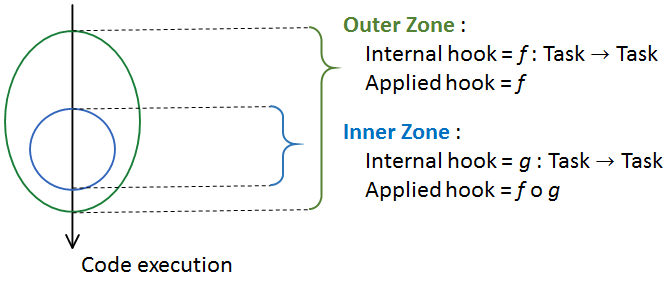
\includegraphics[width=\textwidth]{around-hook}
  \caption{Around hook}
  \label{fig:around-hook}
\end{figure}

\subsection*{Around Hooks Inheritance}

For more flexibility, around hooks are inherited but not repeated. Consider three zones:

\begin{tabular}{|l|l|l|l|}
\hline
\textbf{Zone} & \textbf{Enclosing Zone} & \textbf{Defined hook} & \textbf{Applied hook}
\\\hline
outer Zone & None & $f$: Task $\rightarrow$ Task & $f$
\\\hline
middle Zone & outer Zone & $g$: Task $\rightarrow$ Task & $f \circ g$
\\\hline
inner Zone & middle Zone & $f$: Task $\rightarrow$ Task & $f \circ g$
\\\hline
\end{tabular}

In inner Zone, $f$ hook does not get applied twice, because it would repeat inherited f hook from outer Zone. When the same hook is inherited multiple times, the outermost origin determines its application position. In the previous example, inner Zone applies $( f \circ g )$ and not $( g \circ f )$ because the outermost origin of $f$ (outer Zone) encloses the outermost origin of $g$ (middle Zone). This prevents inner Zones from accidentally modifying inherited hooks application order.

This inheritance policy is more general than a blind straight-forward application of all hooks. It is easy (especially in Java) to re-create a different instance of a hook with the same functionality to prevent it from being filtered out. On the other hand, given a single function composed of many hooks, it is hard, if not impossible, to filter out repetitions to get such union-inheritance.

\section{Realization}
\label{sec:realization}

The hypothesis that any submitted asynchronous code can be hooked permits to safely ignore the Zone integration when discussing its functionalities. The integration will be always possible. This is a great benefit, since it effectively decouples the Zone functional specification from its integration concerns, confronted to the multitude of evolving asynchronous frameworks in Java.

To integrate a Zone in a program, one can see it as a generalization of a Java thread local\footnote{A Java thread local variable has an independently initialized copy unique for each thread}. Note that the concept of thread local is not limited to Java. A mapping from threads to stored values implements the same behavior.

When using a thread pool, the concept of thread local becomes mitigated, even erroneous. Thread locals are bound to a specific thread, but the user does not controls how its tasks are bound to the threads. The common pattern to solve this is to wrap submitted code with instructions that update the thread local for the code.
\begin{lstlisting}

ThreadLocal<T> threadLocal = ...
Executor executor = ...

/*
 * Submitted code will update
 * the thread local on execution.
 */
public void submitWithLocal(Runnable code, T local) {
  Runnable newCode = () -> {
    // saves initial value
    T initial = threadLocal.get();

    // sets desired value for code
    threadLocal.set(local);
    code.run();

    // restores initial value
    threadLocal.set(initial);
  };

  executor.execute(newCode);
}
\end{lstlisting}

The Zone is a generalization of this method. Rather than binding a runnable, any code is accepted, denoted as \emph{task}. The Zone handles internally the thread local to store its reference and simply exports a \lstinline{bind} method.
The Zone takes advantage of this binding operation to apply its internal mechanics and all defined submission hooks. Based on this single binding, it provides:
\begin{itemize}
\item Asynchronous persistent context.
\item Modeled execution flow between the Zones.
\item Flexible programmable hooks on Zone transitions and code submission to the Zone.
\item Extension and reusability mechanisms to extend and implement more Zone features.
\end{itemize}


This pattern efficiently decouples the Zone integration from its functionalities. To use it, one only needs to bind each submitted asynchronous task to the Zone. This can be even simpler using a ``Zone-aware executor'' (see chapter \ref{ch:inpractice} for an example).

Chapter \ref{ch:asyncworld} showed that in Java, one cannot assume a single execution framework. The presented binding solution is not a uniform solution that automagically works in any context. It describes a single operation to execute on every asynchronous submission, which can even be modularized in the execution framework. That is how the Zone gets integrated in programs.
